% Template for PLoS

\documentclass[10pt]{article}
% amsmath package, useful for mathematical formulas
\usepackage{amsmath}
% amssymb package, useful for mathematical symbols
\usepackage{amssymb}
\usepackage{mathpazo}
\usepackage{fontspec}
\setmainfont{Palatino}

% hyperref package, useful for hyperlinks
\usepackage{hyperref}

% graphicx package, useful for including eps and pdf graphics
% include graphics with the command \includegraphics
\usepackage{graphicx}

% Sweave(-like)
\usepackage{fancyvrb}
\DefineVerbatimEnvironment{Sinput}{Verbatim}{fontshape=sl}
\DefineVerbatimEnvironment{Soutput}{Verbatim}{}
\DefineVerbatimEnvironment{Scode}{Verbatim}{fontshape=sl}
\newenvironment{Schunk}{}{}
\DefineVerbatimEnvironment{Code}{Verbatim}{}
\DefineVerbatimEnvironment{CodeInput}{Verbatim}{fontshape=sl}
\DefineVerbatimEnvironment{CodeOutput}{Verbatim}{}
\newenvironment{CodeChunk}{}{}

% cite package, to clean up citations in the main text. Do not remove.
\usepackage{cite}

\usepackage{color}

% Use doublespacing - comment out for single spacing
%\usepackage{setspace}
%\doublespacing


% Text layout
\topmargin 0.0cm
\oddsidemargin 0.5cm
\evensidemargin 0.5cm
\textwidth 16cm
\textheight 21cm

% Bold the 'Figure #' in the caption and separate it with a period
% Captions will be left justified
\usepackage[labelfont=bf,labelsep=period,justification=raggedright]{caption}

% Use the PLoS provided bibtex style
\bibliographystyle{plos}

% Remove brackets from numbering in List of References
\makeatletter
\renewcommand{\@biblabel}[1]{\quad#1.}
\makeatother


% Leave date blank
\date{}

\pagestyle{myheadings}
%% ** EDIT HERE **


%% ** EDIT HERE **
%% PLEASE INCLUDE ALL MACROS BELOW

%% END MACROS SECTION

\usepackage{booktabs}
\usepackage{dcolumn}
\usepackage{rotating}

\begin{document}

% Title must be 150 characters or less
\begin{flushleft}
{\Large
\textbf{SERC Impact Evaluation}
}
% Insert Author names, affiliations and corresponding author email.
\\
  Sneha Patel\textsuperscript{1*},
  Christopher B. Boyer\textsuperscript{1},
  J. Koku Awoonor-Williams\textsuperscript{2},
  Rofina Asuru\textsuperscript{2},
  James F. Phillips\textsuperscript{1}\\
\bf{1} Department of Epidemiology, Columbia University,  New York,  NY,  USA
\\
\bf{2} Regional Health Administration, Ghana Health Service,  Bolgatanga,  Upper East,  Ghana
\\

\textasteriskcentered{} E-mail:   \href{mailto:sp2827@cumc.columbia.edu}{sp2827@cumc.columbia.edu}
  
  
  
  

\end{flushleft}

\section{Model Descriptions}\label{model-descriptions}

We estimate the impact of SERC services using generalized estimating
equations to model change in facility reports of births and rates of
maternal deaths and cesarian sections in the period before and after the
implementation of SERC. Data from SERC facilities are compared to that
of a control group comprised of facilities in neighboring districts in
the Upper East and Upper West Regions of Ghana over the period of
January 2009 to December 2014. Controls were selected from among
facilities with similar socio-demographic and health indicators
statistics in the period prior to the implementation of SERC. Regression
models take the form:

\begin{align}
\mu_{ij} = & \beta_{0} + \beta_{1} x_{ij} + \beta_{2} z_{ij} + \beta_{3} t_{ij} + \beta_{4} (t_{ij} - T_{0})u_{ij} + \beta_{5} x_{ij} z_{ij} + \beta_{6} x_{ij} t_{ij} + \\
           & \beta_{7} z_{ij} t_{ij} + \beta_{8} x_{it} (t_{ij} - T_{0})u_{ij} + \beta_{9} z_{it} (t_{ij} - T_{0})u_{ij} + \nonumber \\
           & \beta_{10} x_{it} z_{ij} t_{ij} + \beta_{11} x_{ij} z_{ij} (t_{ij} - T_{0})u_{ij} + \epsilon_{ij} \nonumber \\
P(\mu | x,z,t) \sim & \textrm{N} [ \mu, \sigma^2 ] \nonumber
\end{align}

and

\begin{align}
\textrm{log} [ \mu_{ij} ] &= \beta_{0} + \beta_{1} x_{ij} + \beta_{2} w_{ij} + \beta_{3} x_{ij} w_{ij} + \epsilon_{ij} \\
P(\mu | x,w) \sim & \textrm{Poisson} [ \mu, \sigma^2 ] \nonumber
\end{align}

where,

\begin{description}
\item[ $\mu_{ij}$ ] The outcome of interest for facility $i$ at time $j$. Note that in the case of c-section and death rates the outcome counts are divided by the total number of births at facility $i$ at time $j$. 
\item[ $x_{ij}$ ] Discrete dummy variable indicator of whether facility $i$ belongs to the treatment or control group.
\item[ $z_{ij}$ ] Discrete dummy variable indicator of whether facility $i$ is a hospital or lower-level facility.
\item[ $t_{ij}$ ] Integer count of months since start of observation period (Jan 1 2009).
\item[ $T_{0}$ ] Time of start of SERC exposure (Aug 1 2013).
\item[ $u_{ij}$ ] Step function which is equal to $0$ if $t_{ij} < T_{0}$ and is equal to $1$ if $t_{ij} \geq T_{0}$.
\item[ $w_{ij}$ ] Discrete variable indicator of whether observation $j$ is pre- or post-intervention.
\item[ $\epsilon_{ij}$ ] Error term for facility $i$ at time $j$. 
\end{description}

Model (1) is used to estimate the number of deliveries recorded by all
359 facilities over 70 months of observation. Model (2) is used to
estimate the rates of cesarean deliveries and maternal deaths among the
17 district hospital facilities that provide these services over 70
months of observation. Repeated observations within a facility are
adjusted for by assuming an exchangeable correlation structure. For
inference, we report robust standard errors obtained via the sandwich
operator.

\section{Results}\label{results}

\begin{CodeChunk}

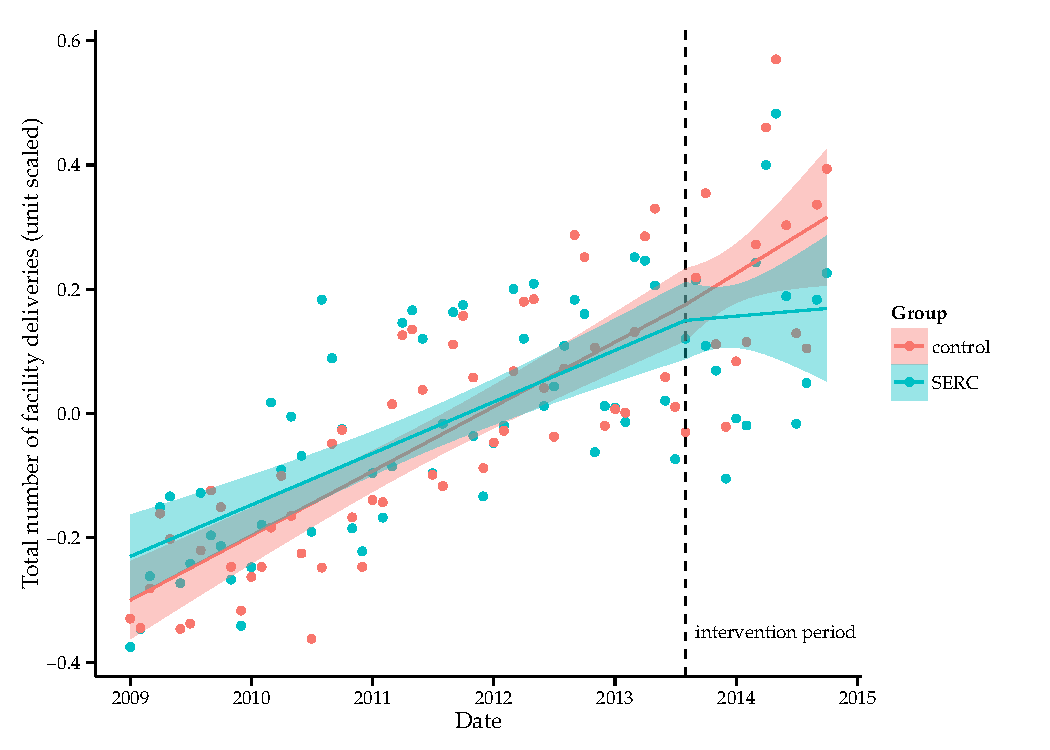
\includegraphics{model_description_files/figure-latex/unnamed-chunk-2-1} \end{CodeChunk}

Figure 1: Plot of total monthly deliveries by intervention group for 359
facilities, UER and UWR, Ghana 2009 to 2015

\begin{CodeChunk}


\begin{center}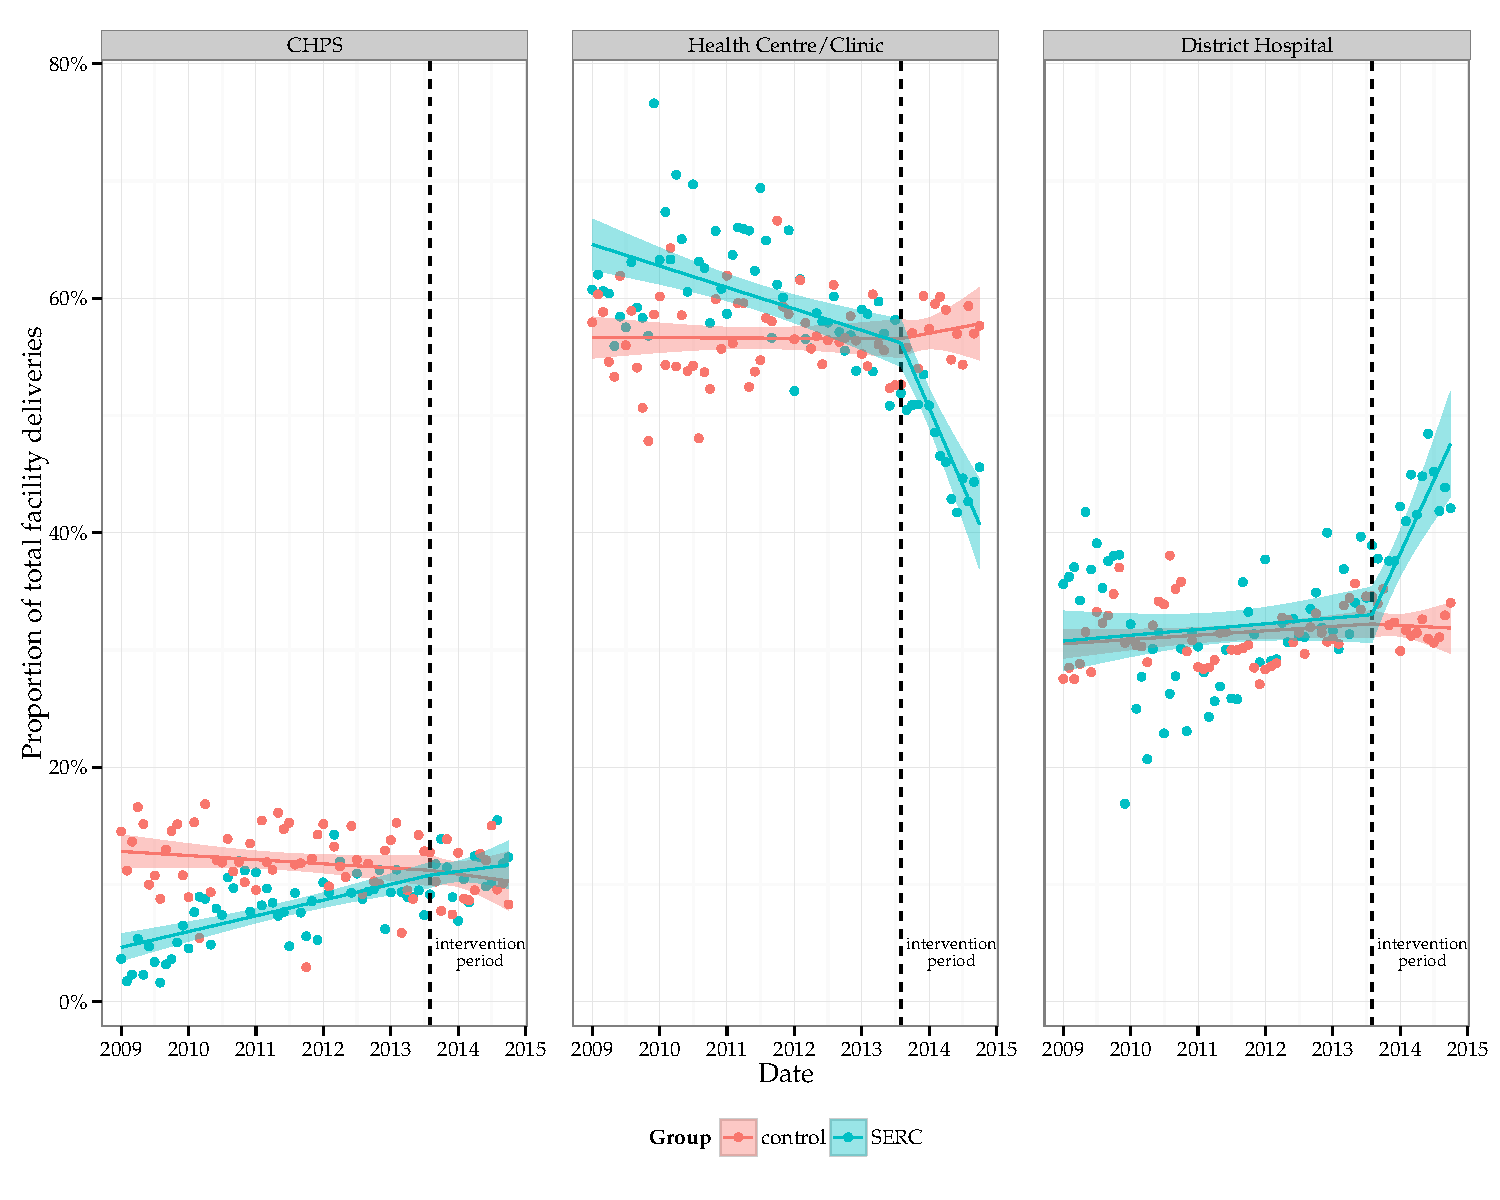
\includegraphics[width=6.5in,height=5.2in]{model_description_files/figure-latex/unnamed-chunk-3-1} \end{center}

\end{CodeChunk}

\begin{sidewaystable}[!htbp] \centering 
  \caption{Summary of GEE models for births and cesarean section, maternal mortality, and infant mortality rates in SERC vs. control districts in Ghana, 2009 - 2015.} 
  \label{} 
\begin{tabular}{@{\extracolsep{0pt}}lcccc} 
\\[-1.8ex]\hline 
\hline \\[-1.8ex] 
 & \multicolumn{4}{c}{\textit{Dependent variable:}} \\ 
\cline{2-5} 
\\[-1.8ex] & births & CSR\textsuperscript{a} & MMR\textsuperscript{b} & IMR\textsuperscript{c} \\ 
\\[-1.8ex] & \textit{normal generalized} & \textit{Poisson generalized} & \textit{Poisson generalized} & \textit{Poisson generalized} \\ 
 & \textit{estimating equation} & \textit{estimation equation} & \textit{estimation equation} & \textit{estimation equation} \\ 
\\[-1.8ex] & (1) & (2) & (3) & (4)\\ 
\hline \\[-1.8ex] 
 \textit{Intercept} & 12.13$^{***}$ (8.74, 15.52) & $-$2.28$^{***}$ ($-$2.67, $-$1.89) & $-$5.79$^{***}$ ($-$6.03, $-$5.55) & $-$3.84$^{***}$ ($-$4.18, $-$3.51) \\ 
  Clinic & $-$2.59 ($-$6.63, 1.44) &  &  &  \\ 
  Hospital & 27.85$^{*}$ ($-$1.94, 57.64) &  &  &  \\ 
  SERC & $-$9.74$^{***}$ ($-$14.16, $-$5.33) & $-$0.20 ($-$0.65, 0.25) & 0.70$^{***}$ (0.36, 1.03) & $-$0.25 ($-$0.61, 0.11) \\ 
  time (\textit{cont}) & $-$0.09$^{***}$ ($-$0.14, $-$0.05) &  &  &  \\ 
  intervention time (\textit{cont}) & 0.04 ($-$0.16, 0.24) &  &  &  \\ 
  Clinic $\cdot$ SERC & 14.21$^{***}$ (7.33, 21.10) &  &  &  \\ 
  Hospital $\cdot$ SERC & 5.61 ($-$24.39, 35.61) &  &  &  \\ 
  Clinic $\cdot$ time & 0.14$^{***}$ (0.08, 0.20) &  &  &  \\ 
  Hospital $\cdot$ time & 0.94$^{***}$ (0.66, 1.22) &  &  &  \\ 
  SERC $\cdot$ time & 0.10$^{***}$ (0.04, 0.16) &  &  &  \\ 
  Clinic $\cdot$ intervention & 0.06 ($-$0.16, 0.28) &  &  &  \\ 
  Hospital $\cdot$ intervention & $-$0.45 ($-$1.14, 0.24) &  &  &  \\ 
  SERC $\cdot$ intervention & $-$0.10 ($-$0.34, 0.13) &  &  &  \\ 
  Clinic $\cdot$ SERC $\cdot$ time & $-$0.07 ($-$0.20, 0.05) &  &  &  \\ 
  Hospital $\cdot$ SERC $\cdot$ time & $-$0.48$^{***}$ ($-$0.83, $-$0.14) &  &  &  \\ 
  Clinic $\cdot$ SERC $\cdot$ intervention & $-$0.39$^{**}$ ($-$0.78, $-$0.01) &  &  &  \\ 
  Hospital $\cdot$ SERC $\cdot$ intervention & 1.78$^{***}$ (0.73, 2.82) &  &  &  \\ 
  period (\textit{cat}) &  & 0.15$^{*}$ ($-$0.01, 0.31) & $-$0.30 ($-$0.77, 0.16) & $-$0.88$^{**}$ ($-$1.66, $-$0.10) \\ 
  SERC $\cdot$ period &  & 0.14 ($-$0.12, 0.39) & $-$0.88$^{*}$ ($-$1.85, 0.09) & 0.08 ($-$1.02, 1.17) \\ 
 \hline \\[-1.8ex] 
Observations & 12,037 & 663 & 731 & 349 \\ 
\hline 
\hline \\[-1.8ex] 
\textit{Note:}  & \multicolumn{4}{l}{$^{*}$p$<$0.1; $^{**}$p$<$0.05; $^{***}$p$<$0.01} \\ 
 & \multicolumn{4}{l}{\textsuperscript{a} Cesarean section rate. Defined as number of cesarean sections divided by the number of births.} \\ 
 & \multicolumn{4}{l}{ \textsuperscript{b} Maternal mortality ratio (facility-based). Defined as the number of maternal deaths per 100,000 live facility births} \\ 
 & \multicolumn{4}{l}{\textsuperscript{c} Infant mortality ratio (facility-based). Defined as the number of infant deaths (0q1) per 1,000 live facility births.} \\ 
\end{tabular} 
\end{sidewaystable}

\end{document}

